%En stokastisk proces i det diskrete tilfælde er en samling af diskrete stokastiske variabler, der har værdier i en mængde, som kaldes \textbf{tilstandsrum}. Mængden er indekseret af \textbf{indeksmængden}, hvor det er typisk de naturlig tal, der anvendes. 
Dette afsnit bygger på \cite{sandsynlighedsBog} og \cite{grimsandsynlighedsBog}.
Et eksempel på en stokastisk proces er den såkaldte forgrenings process, som modellere et ``et-kønnet'' stamtræ, teorien stammer oprindeligt England, hvor Francis Galton, ønskede at undsøge hvilke efternavne, som ville uddø. Processen kan bruges til at modellere mange forskellige stokastiske phenomener, eksempelvis virus, jordskælv og fission.
Lad de diskret stokastiske variable $X_{n,k}$ betegne antallet af \textbf{afkom} den $k$'te forfader i den $n$'te \textbf{generation} får og lad dem være iid med pmf $p_X$. Den første forfader $Z_0$ kaldes \textbf{stamforfaderen}.
Størrelsen på hver generation, betegnet $Z_n$, danner en følge, som kaldes en stokastisk forgreningsproces eller en Galton-Watson proces.
\begin{defn}\label{def:forgreningsproces}
Lad $X_{n,k}$ være iid diskret stokastiske variable med udfaldsrum i $\N_0$ og pmf $p_X$. En \textbf{forgreningsproces} er en følge $\{Z_n\}_{n\geq 0}$ beskrevet ved følgende induktion
\begin{align*}
    Z_n=\begin{cases}
        1&n=0\\
        \sum_{k=1}^{Z_{n-1}}X_{n,k}&n>0,Z_{n-1}>0\\
        0&n>0,Z_{n-1}=0
        \end{cases}
\end{align*}
Fordelingen givet ved $p_X$ kaldes for \textbf{afkomsfordelingen}.
\end{defn}

Et eksempel på en forgeningsproces kan ses i figur \ref{fig:eksforgreningsproces}, som viser et stamtræ for en slægt, hvor stamforfaderen fik to børn $A$ og $B$, som videre fik deres egen slægt $A$ og $B$.

\begin{figure}[H] 
 \centering
    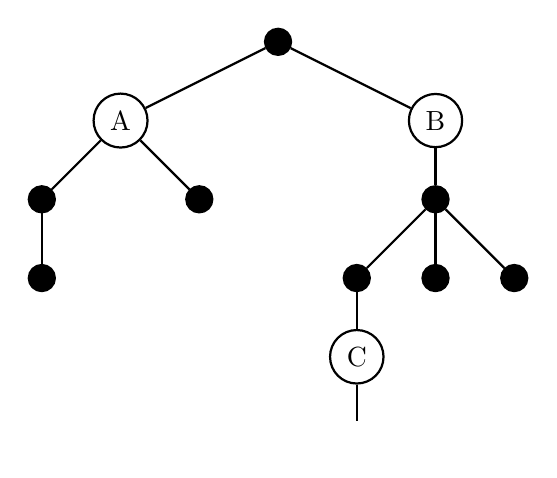
\begin{tikzpicture}
    \tikzset{punkt/.style={circle,thick, draw=black, minimum width=0.1cm,fill=black}}
    \tikzset{punkd/.style={circle,thick, draw=white, minimum width=0.1cm,fill=white}}
    \tikzset{punkta/.style={circle,thick, draw=black, minimum width=0.1cm}}

%Z_0
    \node[punkt] at (0.0, 3.0) (z_1) {};
    
    
%Z_1    
    \node[punkta] at (-2.0, 2.0) (z_21) {A};
    \node[punkta] at (2.0, 2.0) (z_22) {B};
    \draw [-, thick, draw=black] (z_1) -- (z_21);
    \draw [-, thick, draw=black] (z_1) -- (z_22);
%Z_2
    \node[punkt] at (-1.0, 1.0) (z_312) {};
    \node[punkt] at (-3.0, 1.0) (z_311) {};
    \draw [-, thick, draw=black] (z_21) -- (z_312);
    \draw [-, thick, draw=black] (z_21) -- (z_311);
    
    \node[punkt] at (2.0, 1.0) (z_321) {};
    \draw [-, thick, draw=black] (z_22) -- (z_321);
%Z_3
    \node[punkt] at (-3.0, 0.0) (z_411) {};
    \draw [-, thick, draw=black] (z_311) -- (z_411);
    
    \node[punkt] at (3.0, 0.0) (z_413) {};
    \node[punkt] at (2.0, 0.0) (z_412) {};
    \node[punkt] at (1.0, 0.0) (z_411) {};
    \draw [-, thick, draw=black] (z_321) -- (z_413);
    \draw [-, thick, draw=black] (z_321) -- (z_412);
    \draw [-, thick, draw=black] (z_321) -- (z_411);
%Z_4
    \node[punkta] at (1.0, -1.0) (z_511) {C};
    \draw [-, thick, draw=black] (z_411) -- (z_511);

    \node[punkd] at (1.0, -2.0) (z_611) {};
    \draw [-, thick, draw=black] (z_511) -- (z_611);
    
    \end{tikzpicture}
  \caption{En forgreningsproces, hvor $Z_0=1, Z_1=2, Z_2=3, Z_3=4$, $Z_4=1$}
  \label{fig:eksforgreningsproces}
\end{figure}
Et yderligere begreb omkring generationer \textbf{familie}, hvilket er mængden af afkom i generation $(n+1)$ hvert afkom fra genreationen $(n)$ får. Denne mængde kan er selvfølglig tom, hvis afkommet ingen afkom før. I eksempelet er $A$ og $B$ en familie, da de er de to afkom af $Z_0$. Yderligere bliver $Z_1$ der dannet $2$ familier, $Z_2$ danner også $2$ familier, og $Z_3$ danner $1$.

\begin{prop}\label{prop:pgfforgreningsproces}
Lad $\{Z_n\}_{n\geq 0}$ være en forgreningsproces og lad $G$ være pgf til afkomstfordelingen. Da er pgf'er $G_n$ for $Z_n$ givet ved
\begin{align*}
    G_n(s)=
    \begin{cases}
        s & n=0\\
        G_{n-1}(G(s)) & n>0
    \end{cases}
\end{align*}
\end{prop}
\begin{proof}
Det vides, at $Z_0\equiv 1$, altså har $Z_0$ kun et udfald.
Det eneste ikke-nul led i summen fra definitionen af pgf \ref{pgf} bliver da $k=1$, hvilket giver at $G_0(s)=s$.\\
%For $Z_1$ gælder det at $Z_1=\sum_{k=1}^{Z_0}X_{1,k}=X_{1,1}$, altså har $Z_1$ pgf $G$.
For $n>0$ anvendes Galton-Watson formlen fra proposition \ref{prop 3.39} direkte med $N = Z_{n - 1}$.
\end{proof}
\begin{rem}
    Det gælder for notation for pgf'er, at $G=G_1$
\end{rem}
Det kan være interessant at undersøge om en slægt vil uddø på et tidspunkt, og denne hændelse defineres på en følgende måde. 
\begin{defn}%Extinction
    Lad $\{Z_n\}_{n\geq 0}$ være en forgreningsproces.
    Hændelsen, hvor forgreningsprocessen uddør, noteres $\Omega$ og defineres som
    \begin{align*}
        \Omega = \bigcup_{n=0}^\infty\{Z_n=0\}
    \end{align*}
\end{defn}

I figur \ref{fig:eksforgreningsproces}, uddør barn $A$'s slægt i generation $Z_4$, mens nogle af barn $B$'s børnebørn ikke får afkom og deres slægter uddør, dog fortsætter slægt $B$ igennem $C$'s slægt.

\begin{lem}
    Lad $\{Z_n\}_{n\geq 0}$ være en forgreningsproces. Så gælder det, at
    \begin{align*}
        \Omega = \left\{\lim_{n\rightarrow\infty}Z_n = 0\right\}
    \end{align*}
\end{lem}
\begin{proof}
    Fra definition \ref{def:forgreningsproces} ses, at $Z_n=0\implies Z_{n+1}=0$, hvilket giver $\{Z_n=0\}\subseteq\{Z_{n+1}=0\}$. Ved induktion ses det herfra, at
    \begin{align*}
        \forall k\geq 0:\bigcup_{n=0}^k\{Z_n=0\}=\{Z_{k}=0\}
    \end{align*}
    Lader vi $k\rightarrow\infty$ opnås det ønskede resultat
    \begin{align*}
        \Omega=\bigcup_{n=0}^\infty\{Z_n=0\}=\left\{\lim_{n\rightarrow\infty}Z_n = 0\right\}
    \end{align*}
\end{proof}

Sandsynligheden for at forgreningsprocessen uddør er givet som grænseværdien af pgf'ernes værdier i $0$.
\begin{prop}
Lad $\{Z_n\}_{n \geq 0}$ være en forgreningsproces og lad $Z_n$ have pgf $G_n$. Sandsynligheden for, at forgreningsprocessen uddør, er givet ved
\begin{align*}
    P(\Omega)=\lim_{n\rightarrow\infty}G_n(0)
\end{align*}
\end{prop}
\begin{proof}
\begin{align*}
    P(\Omega)&=P\left(\lim_{n\rightarrow\infty}Z_n = 0\right)\\
    &=\lim_{n\rightarrow\infty}P(Z_n = 0)\\
    &=\lim_{n\rightarrow\infty}G_n(0)
\end{align*}
jævnfør proposition \ref{prop:pgfI0Og1}.
\end{proof}

En hurtig måde til at finde sandsynligheden for, at forgreningen uddør er at kigge på fikspunktet $s=G(s)$  
\begin{prop} \label{prop:prop8.7}%8.7
Lad afkomsfordelingen af en forgreningsproces have pgf $G$. Så er den mindste løsning til $s=G(s)$ i intervallet $s\in[0,1]$ givet ved $q=P(\Omega)$.
\end{prop}
\begin{proof}
Først vises det at $q$ er en løsning, hvorefter det vises at det er den mindste løsning.
Lad $X$ være antallet af afkom stamforfaderen får.
Hvis $X=k$, så eksisterer der $k$ uafhængige forgreningsprocesser, der skal uddø, for at slægten uddør.
Sandsynligheden, for at dette sker, er $q^k$, da forgreningsprocesserne er uafhængige af hinanden.
Dette giver, at 
\begin{align*}
    q=\sum_{k=0}^{\infty}P(\Omega|X=k)P(X=k)=\sum_{k=0}^{\infty}q^kP(X=k)=G(q)
\end{align*}
jævnfør sætning \ref{thm:LTP} og det ses, at $P(\Omega)=q$ løser $s=G(s)$.\\ 
Antag nu at der er en anden løsning $r\in[0,1]$.
Fra proposition \ref{prop:pgfforgreningsproces} har vi at
\begin{align*}
    r=G_0(r)=G_0(G(r))=G_1(r)=\dots=\lim_{n\to\infty}G_n(r)
\end{align*}
Da pgf'er er voksende jævnfør korollar \ref{cor:egenskaberVedPGF}, og $r\geq 0$, så er
\begin{align*}
    r = \lim_{n\to\infty}G_n(r) \geq \lim_{n\to\infty}G_n(0)=P(\Omega)=q
\end{align*}
og hermed er $q$ den mindste løsning til $s=G(s)$.
\end{proof}

Den forventede værdi af afkom kan benyttes til at undersøge sandsynligheden for at slægten uddør.
\begin{prop} \label{prop:prop8.9}%8.9
  Lad en forgreningsproces $\{Z_{n}\}_{n \geq 0}$ have en forventede værdi $\mu$ af afkomsfordelingen, $p_{X}$. Hvis $\mu > 1$, så er $P(\Omega) < 1$, ellers hvis $\mu \leq 1$ og $p_{X}(0) > 0$, så er $P(\Omega) = 1$.
\end{prop}
\begin{proof}
  Det vides at $G_{X}$ er en voksende og konveks funktion jævnfør korollar \ref{problem133}.
  Antag $\mu \leq 1$ og $p_{X}(0) > 0$, så er $G_{X}$ voksende fra $G_{X}(0) = p_{X}(0) > 0$ til $G(1) = 1$, jævnfør proposition \ref{prop:pgfI0Og1}. Dette medfører at den mindste løsning til $s = G_{X}(s)$, givet ved $s = 1$, heraf følger det at $P(\Omega) = 1$, jævnfør proposition \ref{prop:prop8.7}.
  Antag nu at $\mu > 1$, så må $G_{X}(s)$ krydse linjen $y = s$, da $G_{X}'(1) = \mu > 1$, jævnfør \ref{prop 3.37} og $G_{X}$ er voksende. Altså eksistere $s < 1$ således $s = G_{X}(s)$, heraf følger det at $P(\Omega) = s$, jævnfør proposition \ref{prop:prop8.7}.
\end{proof}

%\begin{proof} % GAMELT BEVIS
%    Fra proposition \ref{prop 3.37} gælder det, at $\mu=G'(1)$. Hvis $p_X(0)=0$, så er $\mu > 1$, såfremt $\exists n \in \N, n > 1: p_{X}(n) > 0$ og $P(\Omega)=0$. Bemærk at beviset for specialtilfældet, hvor $G'(s)\equiv 1$ er undladt.
%    \\
%    Hvis $p_{X}(0) = 1$
%    \quad Antag nu at $1 > p_X(0) >0$. Fra korollar \ref{problem133} vides det, at pgf'en $G(s)$ er konveks og voksende. Yderligere så er pgf'en stigende fra $G(0)=p_X(0)>0$ til $G(1)=1$. Hvis $\mu>1$, så må $G(s)$ krydse linjen $y=s$, samt er den første skæringen sandsynligheden, for at slægten uddør, hvilket er skarpt mindre end $1$ jævnfør proposition \ref{prop:prop8.7}.
%    Hvis i stedet $\mu\leq1$, så er der ingen skæring med $y=s$ før $1$, og hermed er sandsynligheden $1$.
%\end{proof}
Figur \ref{fig:proofprop8.9} illustrerer de forskellige tilfælde i proposition \ref{prop:prop8.9}. Den blå graf er $\mu\leq1$, den røde graf er $G(0)=0$, den grønne graf er $\mu>1$, og så er den sorte graf $y=s$. 
\begin{figure}[H]
    \centering
   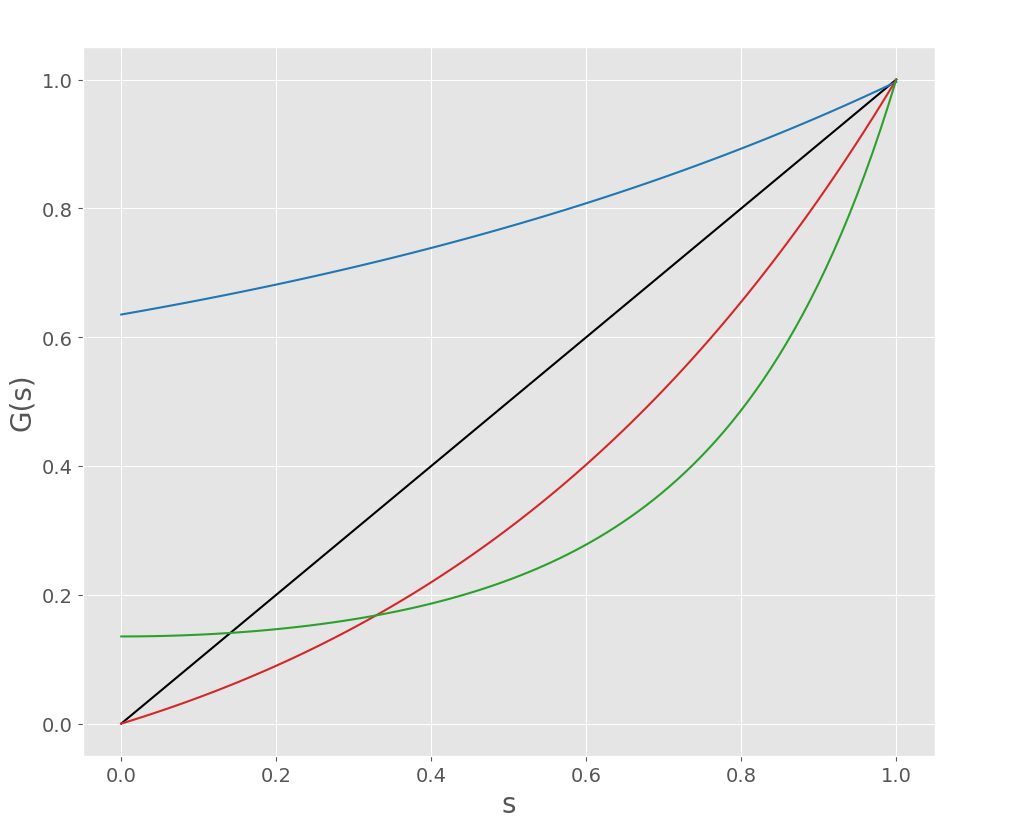
\includegraphics[scale=0.5]{fig/img/Markus.png}
    \caption{Forskellige pgf'er og linjen $y = s$, markeret med sort}
    \label{fig:proofprop8.9}
\end{figure}

\begin{exmp} %Ins fra 8.18
    Betragt en slægt hvor afkomsfordelingen har følgende pmf
    \begin{align*}
        p_X(k) = \begin{cases}
                    3/4  & \text{for } k = 0 \\
                    1/8  & \text{for } k = 1 \\
                    1/8  & \text{for } k = 2 \\
                    0 & \text{ ellers}
                \end{cases}
    \end{align*}
Vi har, at 
\begin{align*}
    G(s)=\frac{3}{4}+\frac{1}{8}s+\frac{1}{8}s^2
\end{align*}
% hvor $G(0)=\frac{3}{4}$. Videre har vi, at
% \begin{align*}
%     G_2(s)=G(G(s))=\frac{3}{4}+\frac{1}{8}\left(\frac{3}{4}+\frac{1}{8}s+\frac{1}{8}s^2\right)+\frac{1}{8}\left(\frac{3}{4}+\frac{1}{8}s+\frac{1}{8}s^2\right)^2
% \end{align*}
% hvor 
% \begin{align*}
%  G_2(0)=\frac{3}{4}+\frac{1}{8}\left(\frac{3}{4}\right)+\frac{1}{8}\left(\frac{3}{4}\right)^2=\frac{3}{4}+\frac{3}{32}+\frac{9}{128}=\frac{117}{128}\approx 0,844   
% \end{align*}
% Hvis dette fortsættes fåes $G_3(0)\approx0.969$, $G_4(0)\approx0.989$, $G_5(0)\approx0.996$, og $G_6(0)\approx0.998$. Hermed vil $P(\Omega)=\lim_{n\to\infty}=1$. 

Fra proposition \ref{prop:prop8.7} vides, at den mindste løsning til $s=G(s)$ er $P(\Omega)$.
\begin{align*}
    s=\frac{3}{4}+\frac{1}{8}s+\frac{1}{8}s^2
\end{align*}
hvor løsningerne til andengradsligningen er $1$ og $6$, hvor $P(\Omega)=1$ så er den mindste løsning til ligningen. 

En anden måde, resultatet kan findes, er ud fra proposition \ref{prop:prop8.9}, da $G'(s)=\frac{1}{8}+2\frac{1}{8}s$, så 
\begin{align*}
    G'(1)=\mu=\frac{1}{8}+2\frac{1}{8}=0.375
\end{align*}
hvilket er mindre end $1$, og hermed er $P(\Omega)=1$
\end{exmp}


\begin{prop} %8.8
Ved en forgreningsproces hvor afkomstfordelingen har forventet værdi $\mu$ og variansen $\sigma^2$, så er $E[Z_n]=\mu^n$ og
    \begin{equation*}
        \Var[Z_n] = \begin{cases} 
        n\sigma^2 & \text{ hvis } \mu =1\\
        \dfrac{\sigma^2(\mu^n-1)\mu^{n-1}}{\mu-1} & \text{ hvis } \mu \neq 1
        \end{cases}
    \end{equation*}
\end{prop}

\begin{proof}
Ved at benytte proposition \ref{prop:cor 3.13} fåes det, at $E[Z_N]=\mu E[Z_{n - 1}]$, heraf fåes
\begin{align*}
    E[Z_n]=\mu E[Z_{n - 1}]=\mu^2E[Z_{n-2}]= \dots = \mu^{n - 1} E[Z_1] = \mu^n
\end{align*}
Vi beviser formlerne for varians ved hjælp af induktion. 
Det gælder, at $\Var[Z_1] = \Var[X] = \sigma^2$, da der kun er et individ til at reproducere.
Benyt proposition \ref{prop:cor 3.13} med $N = Z_{n- 1}$ til at skrive
\begin{align*}
    \Var[Z_n] = E[Z_{n - 1}]\Var[X] + E[X]^2\Var[Z_{n - 1}]  = \mu^{n - 1}\sigma^2 + \mu^2\Var[Z_{n - 1}]
\end{align*}
Antag at $\mu = 1$ og formelen gælder for $\Var[Z_{n - 1}]$, vi har derfor, at 
\begin{equation*}
 \Var[Z_n] = 1^{n-1}\sigma^2 + 1^2 (n - 1)\sigma^2 = n \sigma^2   
\end{equation*}
per vores induktions antagelse.
Antag nu, at $E[X] = \mu \neq 1$, igen har vi, at formelen gælder for $\Var[Z_1]$, da 
\begin{equation*}
    \frac{\sigma^2(\mu - 1)\mu^0}{\mu - 1} = \sigma^2 = \Var[Z_1]
\end{equation*}
Antag derfor, at resultatet gælder for $\Var[Z_{n - 1}]$, så følger det, at
\begin{align*}
    \Var[Z_n] &= \mu^{n - 1} \sigma^2 + \mu^2 \frac{\sigma^2(\mu^{n  - 1} -1)\mu^{n-2}}{\mu-1} \\
    &= \frac{\sigma^2\mu^{n - 1}(\mu - 1)}{\mu - 1} + \frac{\sigma^2(\mu^{n - 1}-1)\mu^{n}}{\mu-1} \\
    &= \sigma^2\frac{\mu^{n - 1}(\mu - 1) + \mu^{n - 2}(\mu^{n - 1} - 1)}{\mu - 1}
    = \sigma^2 \frac{-\mu^{n - 1} + \mu^{2n - 1}}{\mu - 1} = \frac{\sigma^2(\mu^n - 1)\mu^{n - 1}}{\mu - 1}
\end{align*}
hvilket afslutter induktionsskridtet og beviset.
\end{proof}
Vi vil nu undersøge om antallet af individer kan gå imod et $n \in \N$.

\begin{prop} %8.10 (vi mangler bemærkningen under)
Hvis $P(Z_n \to 0) = q$ for $n \to \infty$, så gælder det, at  $P(Z_n \to \infty) = 1 - q$ for $n \to \infty$.
\end{prop}
\begin{proof}
Antag først at $Z_n\not\to\infty$.
Dette betyder, at følgen har en øvre grænse $M$, således at $Z_n \leq M \; \forall n\in \N$.
Generation $Z_{n+1}=0$, hvis ingen individer i forrige generation får afkom, hvilket har sandsynlighed $p_X(0)^{Z_n}\geq p_X(0)^{M}>0$.
Da denne sandsynlighed er positiv for alle $Z_n$, må der efter nok generationer være en generation hvor $Z_n=0$.
Altså gælder det for $n \to \infty$, at $Z_n\not\to\infty\implies Z_n\to0$.
Det gælder også, at $Z_n\to0\implies Z_n\not\to\infty$, så hændelserne er ækvivalente. Med dette konkluderes, at $P(Z_n \to 0) = P(Z_n\not\to\infty) = q \implies P(Z_n\to\infty) = 1-q$ for $n \to \infty$.
\end{proof}

\subsection{Revisted (skal ikke være her, men så har vi har styr på hvad der igang)}

$G(s)=E[s^{Z_1}]$

Lad $T=\inf{n:Z_n=0}$ være generationen, hvor forgreningen uddør. Lad $E_n={n<T<\infty}$
være hændelsen hvor forgreningen uddør efter $n$. 

$p_j(n)=P(Z_n=j | E_n)$

$q_j=lim_{n\to \infty} p_j(n)$


\begin{lem} \label{Lem:lem6.7.1grim}
Hvis $E[Z_1]<\infty$, så $\lim_{n\to \infty} p_j(n)=q_j$ eksistere. 
Så overholder pgf'en 
\begin{align*}
G^{\pi}(s)=\sum_{j=0}^{}q_j s^j 
\end{align*}
at
\begin{align} \label{alg:alg6.7.2grim}
G^{\pi}(\eta^{-1}G(s\eta)=G'(\eta)(G^{\pi}(s)-1)+1   
\end{align}
hvor $\eta$ er sandsynligheden for, at frogreningsproccen uddør
\end{lem}
\begin{proof}
\end{proof}
\begin{rem}
Når $\mu=E[Z_1] \leq 1$, så er $\eta=1$ og $G'(\eta)=\mu$, hvilket leder til, at \eqref{alg:alg6.7.2grim} reducres til 
\begin{align*}
    G^\pi(G(s))=\mu (G^\pi(s)-\mu)+1
\end{align*}
\end{rem}

\begin{cor} \label{cor:cor6.7.7grim}
Lad $\mu=E[Z_1]$. Hvis 
\begin{itemize}
    \item $\mu \neq 1$, så er $\sum_{j=0}^{}q_j=1$. 
    \item $\mu=1$, så er $q_j=0$ for alle $j$. 
\end{itemize}
\end{cor}

\begin{thm} \label{thm:thm6.7.8grim}
Hvis $\mu=E[Z_1]$ og $G''(1)<\infty$, så overholder $Y_n$, at
\begin{align*}
    \lim_{n\to\infty}P(Y_n\leq y|E_n) = 1-e^{-2y}
\end{align*}
\end{thm} 
















